\section{Use Cases}
\label{Use Cases}
Um das Zusammenwirken aller Microservices innerhalb des Hamaube-Systems aufzuzeigen und nachvollziehen zu können, werden im Folgenden einige Use Cases und dazu gehörige Kommunikation vorgestellt, bei denen mehrere Microservices beteiligt sind.

\subsection{User erstellt einen neuen Tweet}
Wenn ein User einen Tweet erstellt (oder ein neuer Tweet über die Twitter API in das Hamaube-System gepusht wird),
wird dieser Tweet über das \textit{USER\_ISSUES\_TWEET} Topic verteilt.
Der Cassandrareader speichert den Tweet, damit dieser später für Hamaube Nutzer angezeigt wird. Nach dem Speichern wird über das Topic \textit{TWEET\_SAVED} eine entsprechende Meldung zurückgegeben, sofern der Tweet erfolgreiche gespeichert wurde.
Nun sind aber noch weiter Microservices an das Topic angebunden. So verarbeitet auch der ElasticSearch Microservice den übermittelten Tweet um ihn z.B. später in Suchanfragen zu berücksichtigen. Und auch der SparkStreaming Microservice verabeitet den Tweet z.B. um Analysen zu erstellen.

\begin{figure}[htbp!]
	\centering
	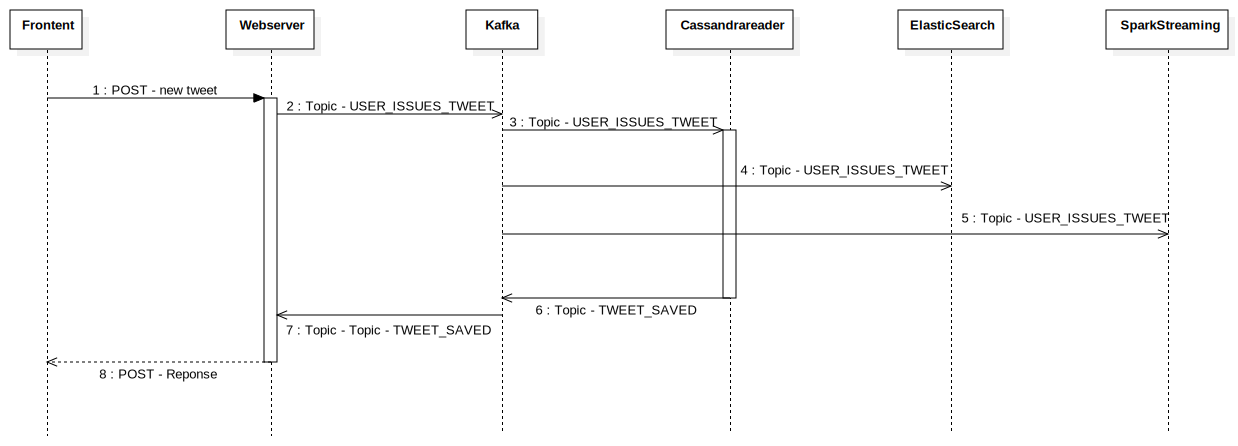
\includegraphics[width=\textwidth]{pics/useCases/IssueTweet}
	\caption{Sequence Diagram: User erstellt neuen Tweet}
\end{figure}

\subsection{User sucht einen Tweet (nach Text)}
Derzeit bietet das Hamaube-System Suchen von Tweets über Hashtags oder über den Tweet-Text.
Im Folgenden wird letzterer Fall betrachtet.
Sobald ein Nutzer im Frontend nach einem Tweet sucht, wird die Suchanfrage über Kafka an den ElasticSearch Microservice weitergereicht. Dieser vermittelt das Ergebnis der Suche als Tweet-IDs über ein Antwort-Topic, welches wiederum an den Cassandrareader geht.
Dieser liest die zugehörigen Tweets aus Cassandra und veröffentlicht das Ergebnis an den WebServer.
Gerade hier zeigt sich, dass die Meta-Information vom ursprünglichen WebServer bis zur letzten Stelle weitergereicht werden müssen, damit auch der richtige WebServer letztendlich die Tweets zur Anfrage erhält.


\begin{figure}[htbp!]
	\centering
	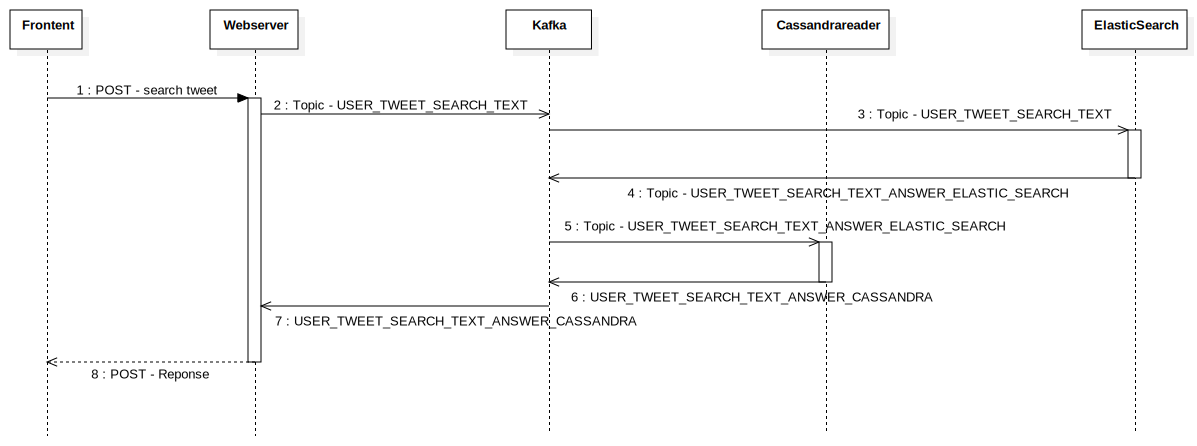
\includegraphics[width=\textwidth]{pics/useCases/SearchTweet}
	\caption{Sequence Diagram: User sucht nach einem Tweet (by text)}
\end{figure}